\newpage
\thispagestyle{empty}
\clearpage\mbox{}\clearpage
\section{Simulation vs schematic comparison}

\subsection{Simulation setup}
Last step was to characterize the layout and evaluate its behaviour in comparison with the schematic. The carried on analysis are the following:
\begin{itemize}
	\item Time domain output mixed signal and spectral components;
	\item Oscillator amplitude to maximize output component;
	\item Conversion gain and 1dB compression point;
	\item Single tone IIP\textsubscript{3};
	\item Two tone IIP\textsubscript{3};
	\item Bandwidth of RF stage (output node filtering of output signal, current mixing);
	\item Static power dissipation;
\end{itemize}
All the analysis were developed using monochromatic signals at frequencies 100MHz for LO, 110MHz for RF, and considering the mixer working in down-conversion (10MHz IF frequency).

To compare schematic and layout we used the set-up proposed in figure \ref{fig:setup}, that includes:
\begin{itemize}
	\item The symbols related to mixer's schematic and layout under test.
	\item Input AC signals generators. Those elements are connected to ideal baluns (figure \ref{fig:balun}) in order to simulate a perfect 50 \(\Omega\) impedance matching condition, producing differential inputs also. Two LO generators are used to customize the optimal carrier power level entering in each mixer.
	\item Power supply net, implicitly connected to both layout and schematic.
	\item Mixer's loads, represented by 50\(\Omega\) resistors connected to unitary gain driven generator. This is used both for ideal impedance matching purposes and to convert differential (balanced) output from mixers to single-ended (unbalanced).
\end{itemize}

\begin{figure}[H]
	\centering %se si cambia posizione a questa immagine assicurarsi che sia girata con il fondo verso il bordo esterno della pagina
	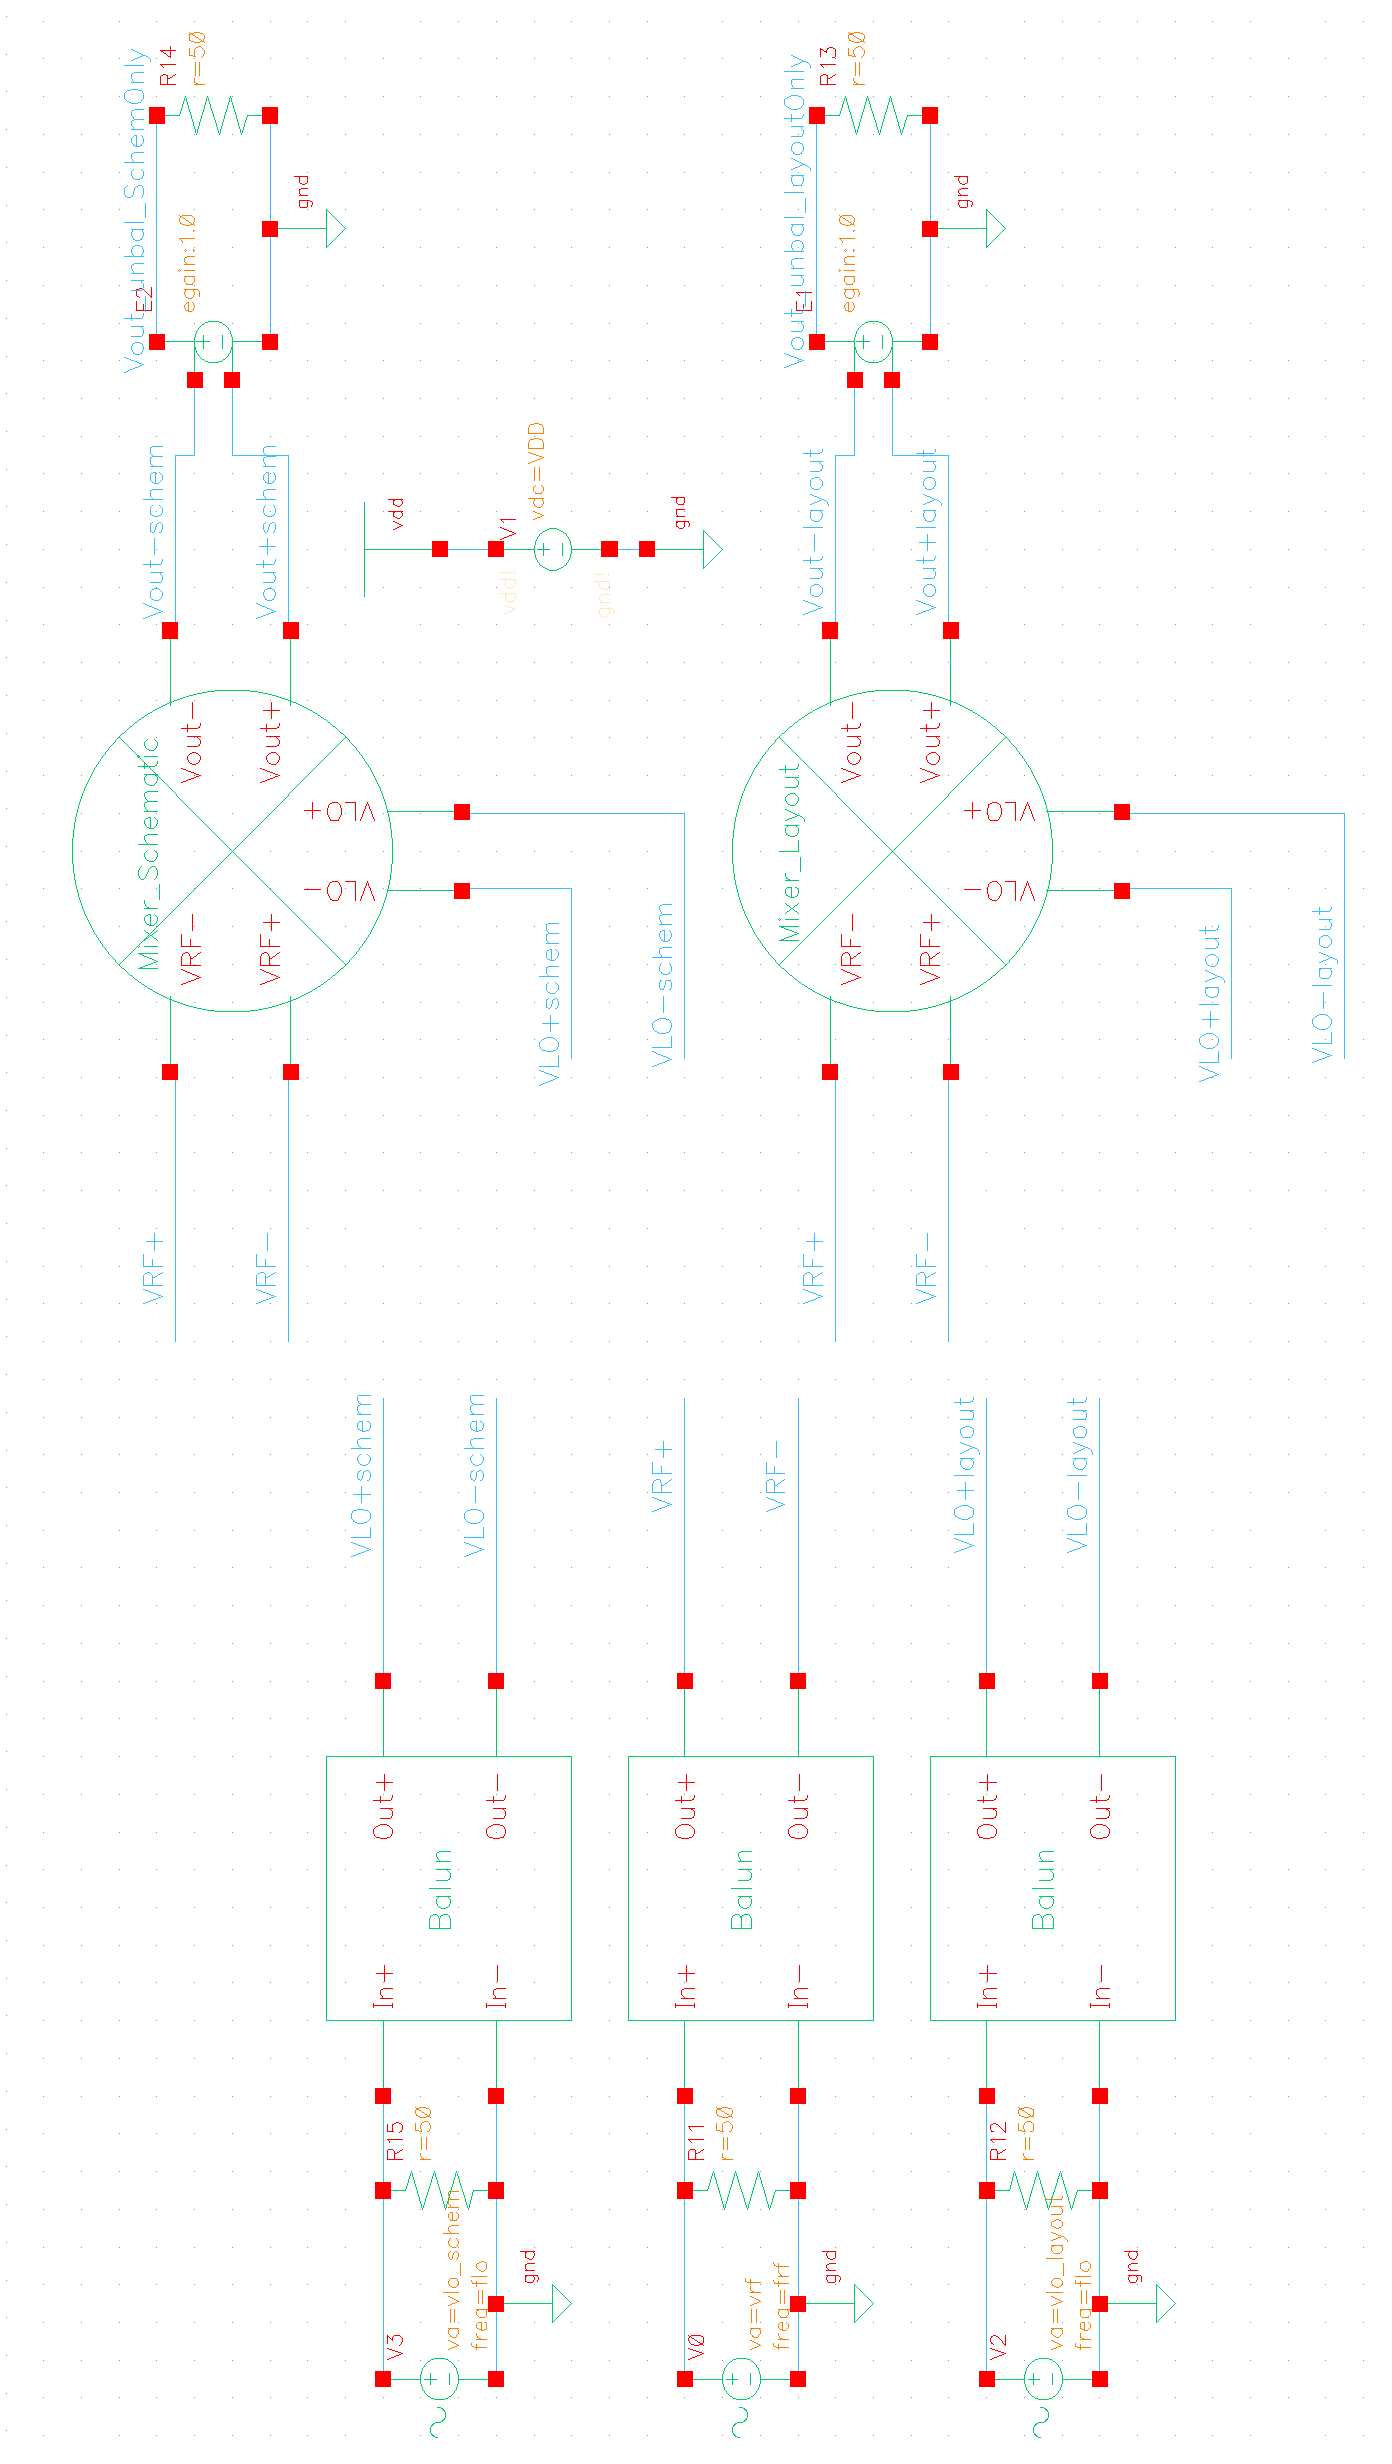
\includegraphics[scale=0.28]{setup}
	\caption{Simulation set-up.}
	\label{fig:setup}
\end{figure}


\begin{figure}[H]
	\centering
	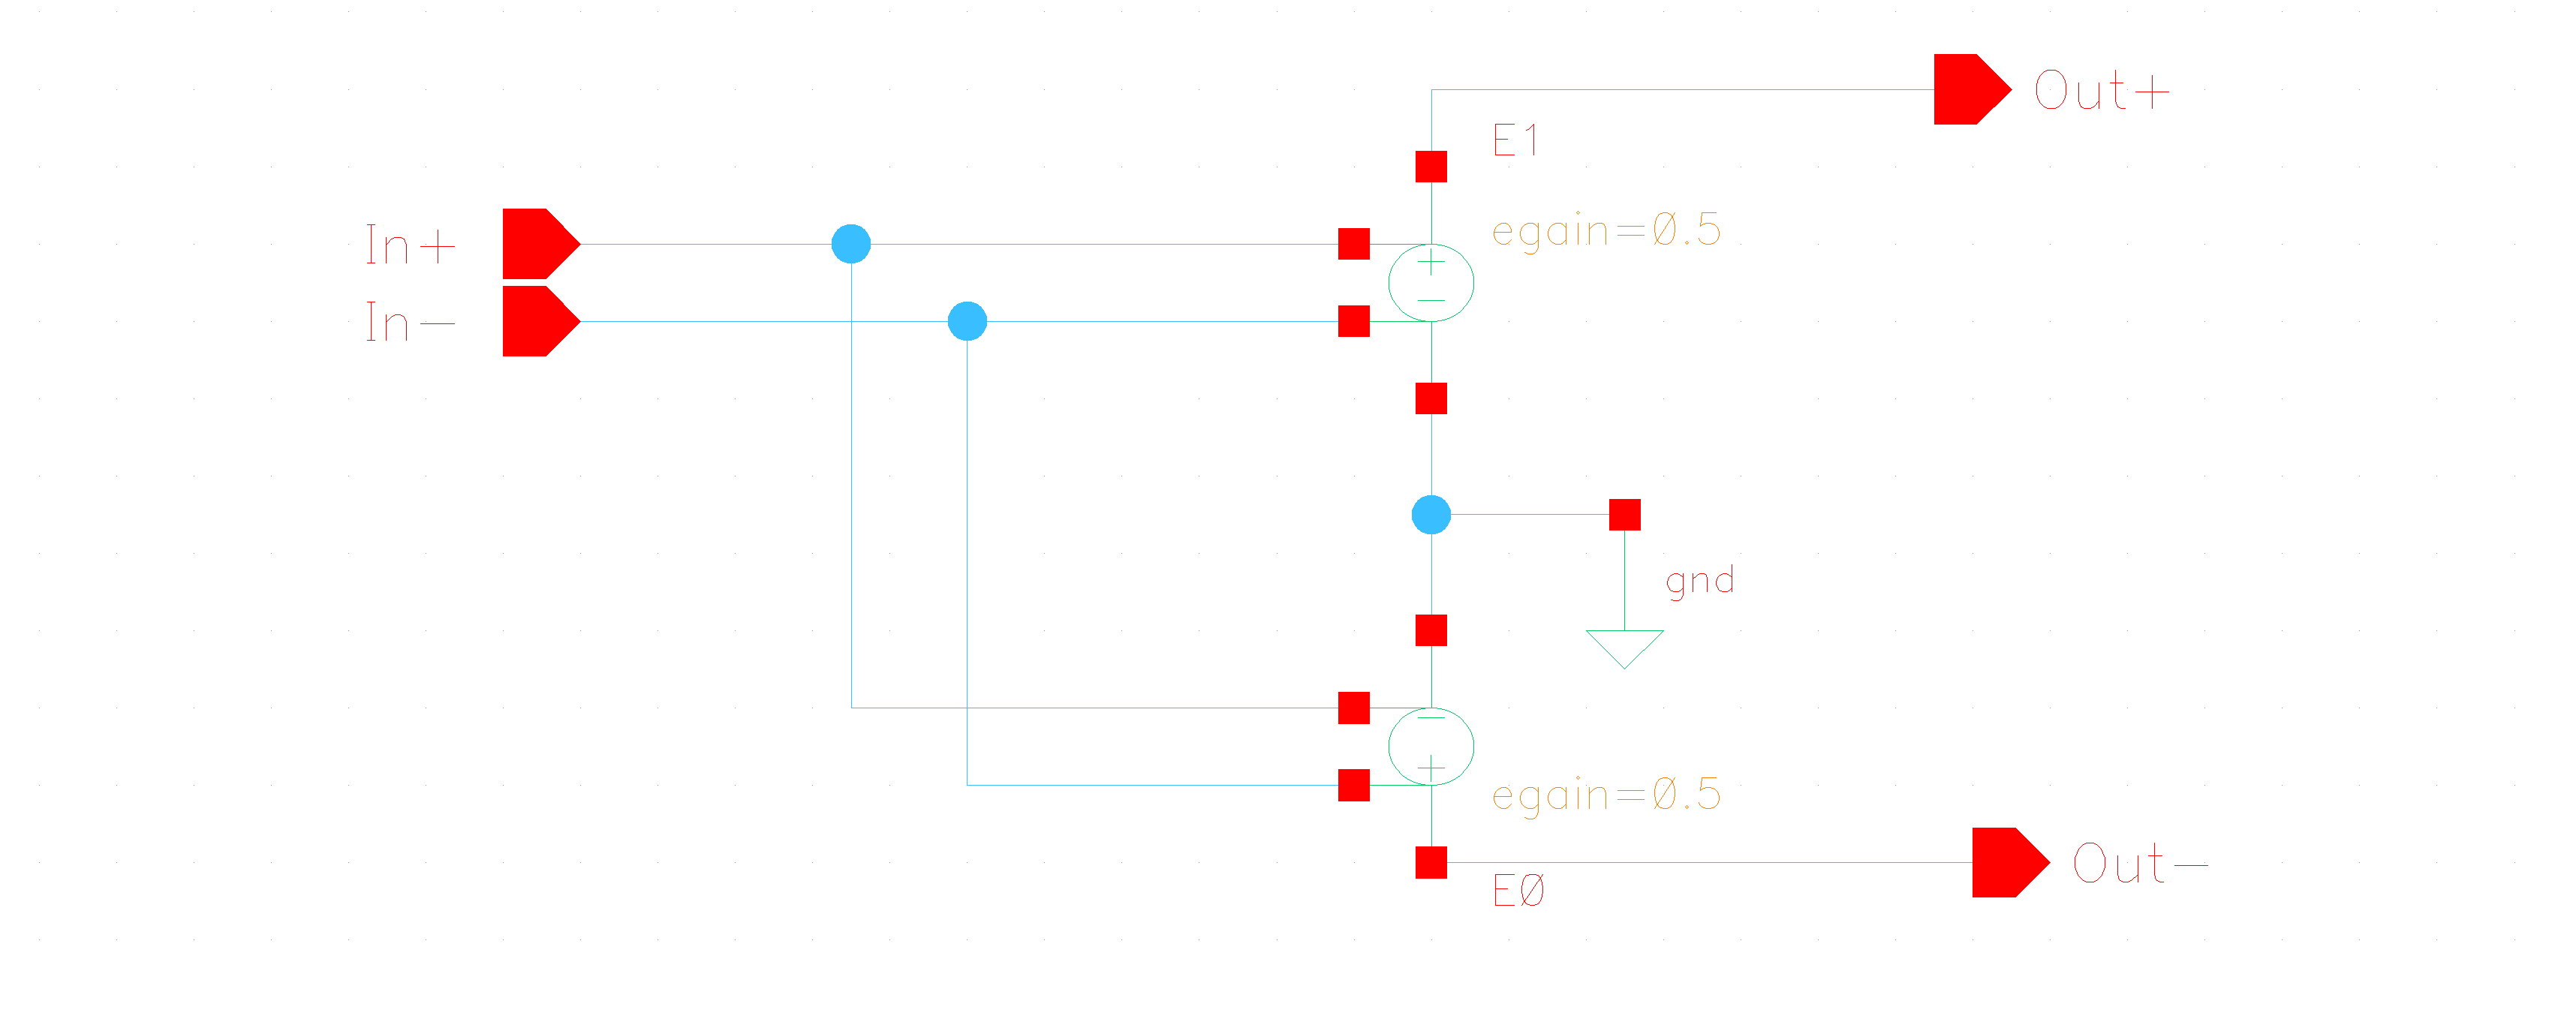
\includegraphics[scale=0.08]{balun}
	\caption{Balun schematic.}
	\label{fig:balun}
\end{figure}

\subsection{Bandwidth evaluation}

Being a mixer a non-linear circuit, we cannot evaluate the bandwidth computing Bode's diagram by means of AC small signal analysis. 
A first, rough, idea about each transistors performances can be obtained by measuring the transition frequency. Current gains have been simulated for both RF and LO stages, whit bias operative condition previously found (figure \ref{fig:bandwidth}a), having:
\begin{gather}
f_T|_{RF}=9.43GHz \notag \\
f_T|_{LO}=1.12GHz \notag 
\end{gather}  
These frequency values are not directly related to the circuit's actual speed, however a limiting upper bound can be used as reference (maximum frequency ten time lower than f\textsubscript{T}). 

Figure \ref{fig:bandwidth}b shows the conversion gain as a function of RF input signal. We set \(f_{LO}=f_{RF}-10\)MHz, in order to keep constant \(f_{IF}\). As it appears our working point presents a small decreasing from maximum gain, it is quite distant from the -3dB point though (almost 2 octaves lower).

If we consider f\textsubscript{-3dB} as the maximum operative frequency we that the circuit presents surprising performance, since this point gets very close to transition frequency. 

However we never considered high frequency reactive behaviour, because the model provided by the CAD tool was not intended to take into account the full set of parasitics, which play an important role at RF. The circuit physical implementation would be surely worse (mainly due to connection and package).

Pretending that our simulation is accurate, this assumption of LO and RF frequency represents the worst case operative condition. 

Our assumptions on LO and RF frequencies were thus considered adequate, since represent the worst-case performances of the mixer.  Maximum operating frequency could thus be improved reducing output node capacitance (for example using a folded cascode configuration for the mixing stage). 
\begin{figure}[H] 
	\centering
	\subfloat[][\emph{current gain}]{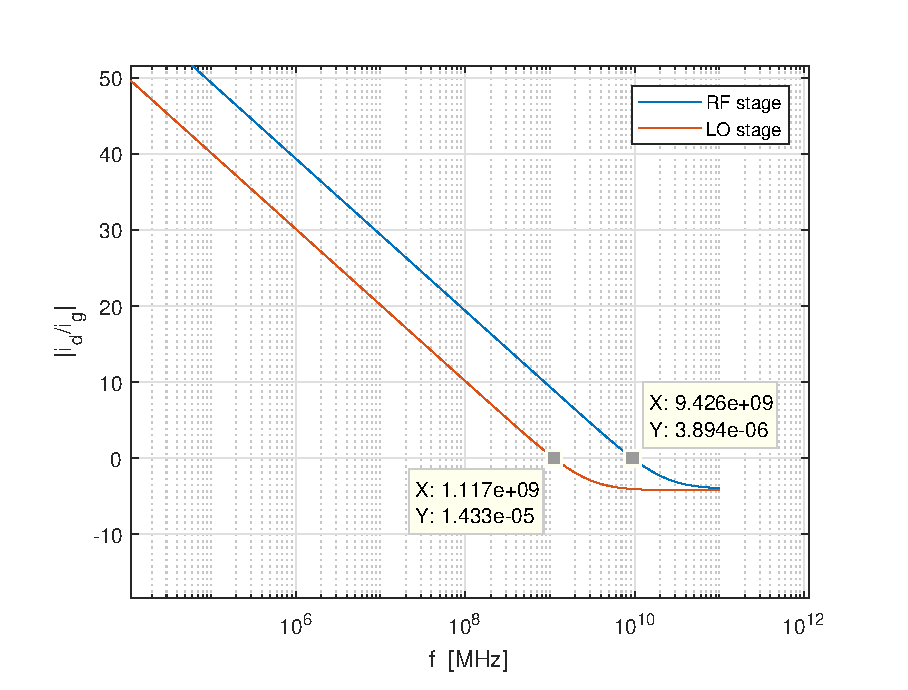
\includegraphics[scale=.75]{transition_freq}} \\
	\subfloat[][\emph{Conversion gain vs bandwidth}]{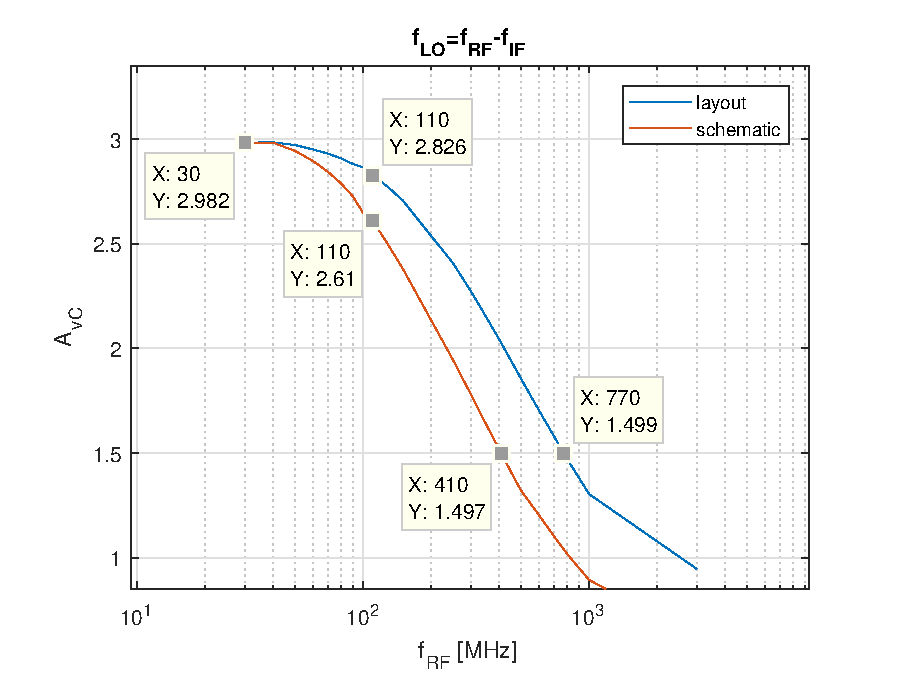
\includegraphics[scale=.75]{bandwidth}}
	\caption{a) transition frequency and b) mixer bandwidth evaluation. In figure b it is possible to identify the constant gain region (f\textsubscript{30MHz}), gain value for this project (f\textsubscript{110MHz})  and -3dB points for RF and LO stages respectively.}
	\label{fig:bandwidth}
\end{figure}


\begin{figure}[H]
	\centering
	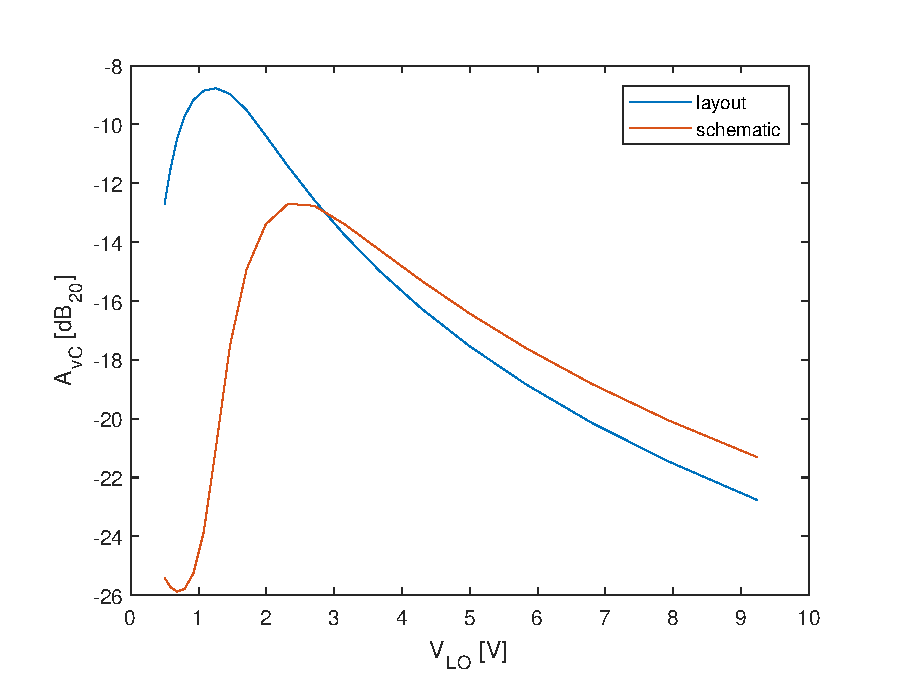
\includegraphics[scale=0.7]{gain_vs_VLO}
	\caption{Conversion gain vs v\textsubscript{LO}.}
	\label{fig:maxGainvsLO}
\end{figure}



\subsection{Maximum conversion gain vs LO}
Input LO signal was swept to find the optimum value that maximizes output voltage at IF. The analysis has been carried on for both schematic and layout circuit. Voltage \(v_{rf}=200mV\) was kept constant during the analysis, and output amplitude at 10MHz was divided by LO amplitude such that the peak corresponds to the maximum LO amplitude for which IF output power saturates. Results are shown in figure \ref{fig:maxGainvsLO}. It can be noticed that schematic and layout reach their maximum for different values of LO signal, \(2.5V\) and \(1.23V\) respectively. 
In general it can be noticed that layout has an higher gain than the schematic. Trying to change \(v_{rf}\) amplitude very tiny changes in peak output voltage where found, so the first analysis was kept as a quite good estimation for optimum LO peak voltage. From now on all the comparison between the two circuits have been made imposing the optimum LO voltage for each circuit.

\begin{figure}[H] 
	\centering
	\subfloat[][\emph{layout}]{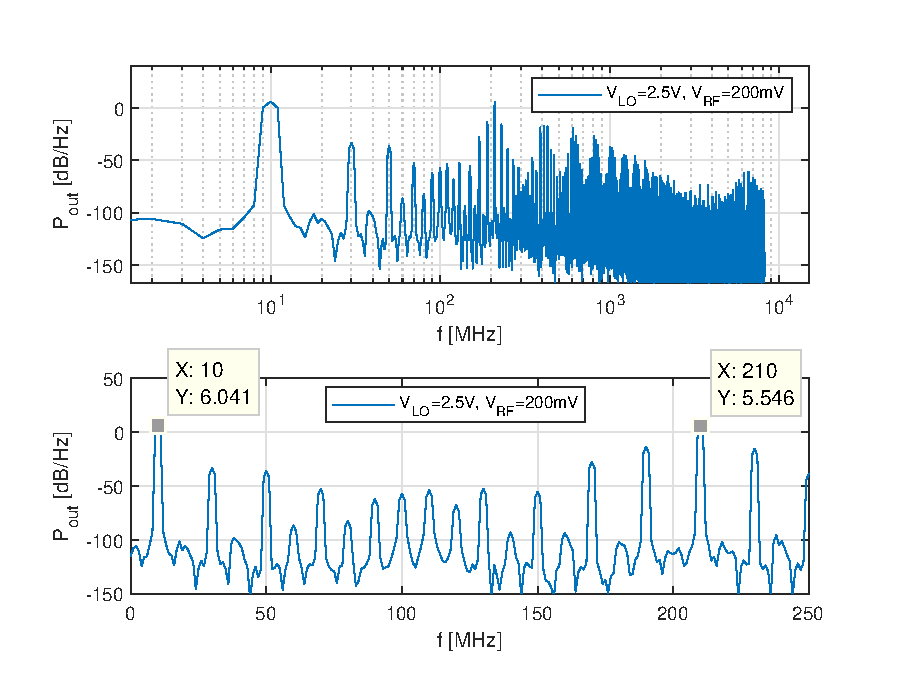
\includegraphics[scale=.75]{DFT_layout}} \\
	\subfloat[][\emph{schematic}]{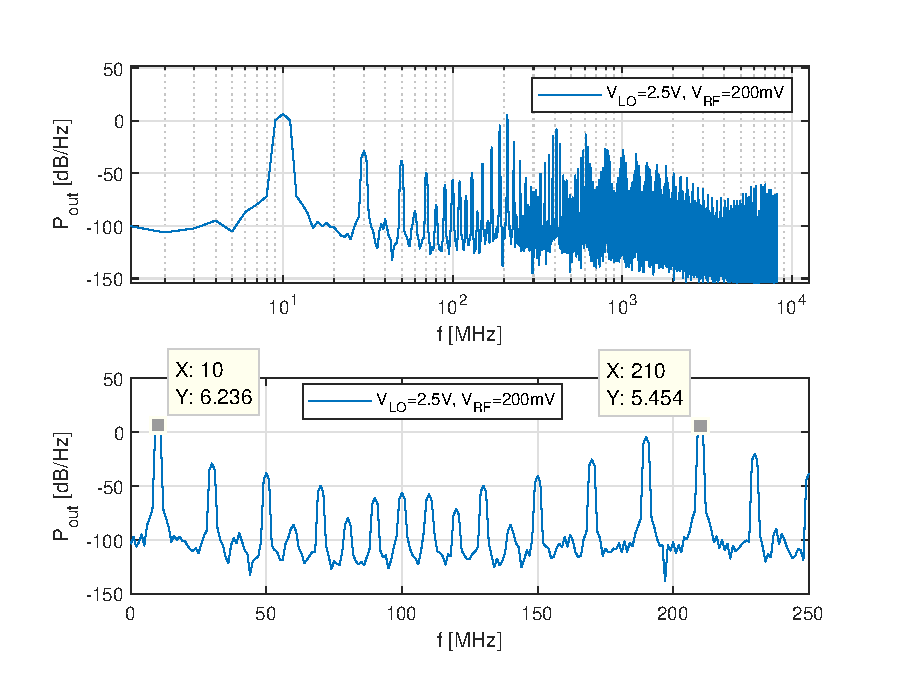
\includegraphics[scale=.75]{DFT_schem}}
	\caption{Discrete Fourier transform: double balanced differential output with v\textsubscript{RF}=200mV,  f\textsubscript{RF}=110MHz, v\textsubscript{RF}=1.23mV, f\textsubscript{LO}=100MHz,cosine squared smoothing function. a) layout, b) schematic}
	\label{fig:TdomaniDFT}
\end{figure}

\begin{figure}[H]
	\centering
	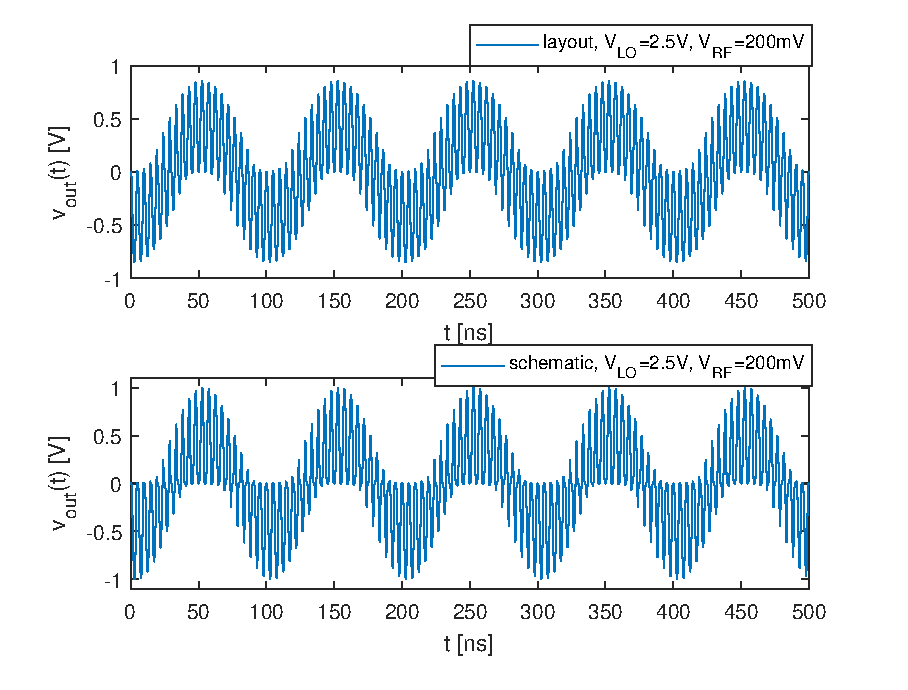
\includegraphics[scale=0.5]{waveforms}
	\caption{Time domain waveforms: double balanced differential output with v\textsubscript{RF}=200mV,  f\textsubscript{RF}=110MHz, v\textsubscript{RF}=1.23mV, f\textsubscript{LO}=100MHz.}
	\label{fig:TdomaniWF}
\end{figure}

\subsection{Time domain mixed signal}
The mixed output signal with \(v_{rf}=\)200mV and \(v_{lo}=\)1.23V is visible in figure \ref{fig:TdomaniWF}. The waveform looks like the expected one from literature.
Applying the discrete Fourier transform to the if signal we found the graph seen in figure \ref{fig:TdomaniDFT}a and \ref{fig:TdomaniDFT}b.
It's clearly visible the intrinsic capability of double balanced mixer of rejecting input components at \(v_{lo}=100\)MHz and \(v_{rf}=\)110MHz.

\subsection{Conversion gain and 1dB compression point}
Keeping optimum LO amplitude, RF's voltage was swept in order to see how output power at IF frequency increases with input power at RF. Reference port for all power measurement has been chosen to be \(50\ohm\). \(P_{IF}\) as a function of \(P_{RF}\) conversion gain is shown in figure \ref{fig:PinPout1T_1dBCp} for both schematic and layout, whereas gain can be seen in figure \ref{fig:GainvsRF}. 
From simulation we have:
\begin{gather}
A_{vC}|_{layout}=2.926 \notag \\ 
A_{vC}|_{schematic}=2.675 \notag
\end{gather}
Extrapolation of 1dB compression point was carried on, leading to the measurement of RF power for which the gain drops of 1dB equal to 
\begin{gather}
P_{RF,in}|_{layout}=-2.3dB_{m} \notag \\
P_{RF,in}|_{schematic}=-4.8dB_{m} \notag
\end{gather}
then, respectively for schematic and layout, corresponding to the voltages:
\begin{gather}
V_{RF,in}|_{layout}=172mV \notag \\
V_{RF,in}|_{schematic}=128mV \notag
\end{gather}



\begin{figure}[H] 
	\centering
	\subfloat[][\emph{P\textsubscript{in}/P\textsubscript{out}}]{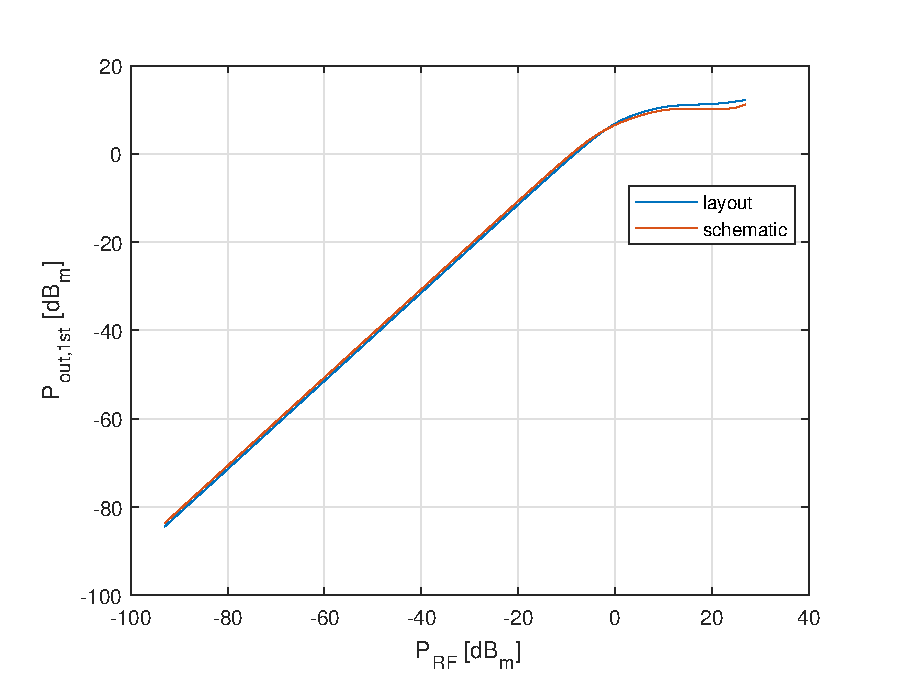
\includegraphics[scale=.75]{pin_pout_VRF}} \\
	\subfloat[][\emph{1dB compression point}]{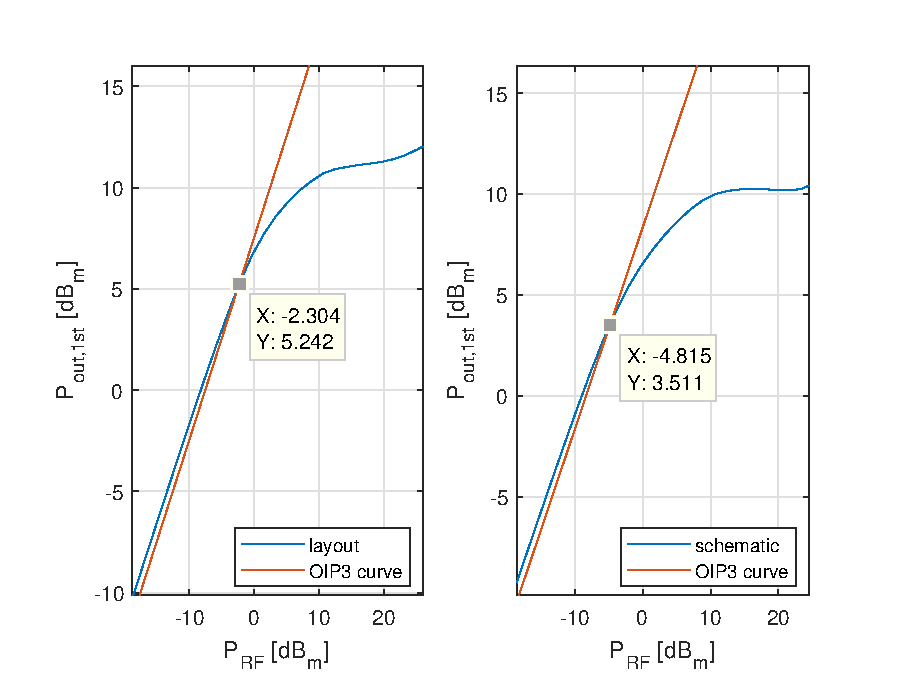
\includegraphics[scale=.75]{1dB_compression_1tone}}
	\caption{a) P\textsubscript{in}/P\textsubscript{out} and  b) 1dB compression point, one-tone analysis.}
	\label{fig:PinPout1T_1dBCp}
\end{figure}


\begin{figure}[H]
	\centering
	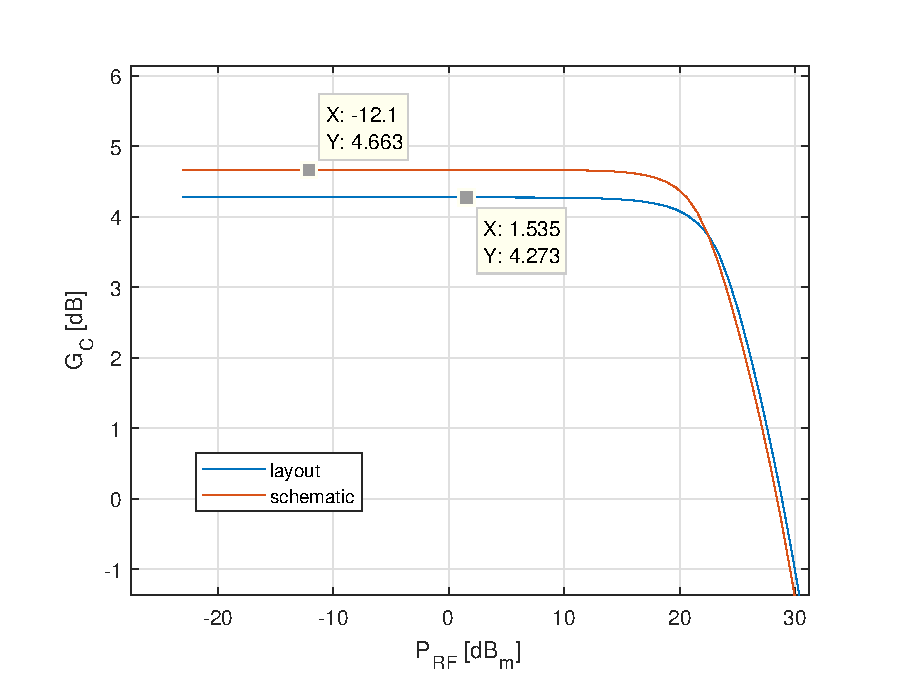
\includegraphics[scale=0.75]{gain_vs_VRF}
	\caption{Conversion gain vs v\textsubscript{RF}.}
	\label{fig:GainvsRF}
\end{figure}


\subsection{Single tone third order distortion}
Using single tone RF signal, power on the third harmonic with respect to the IF tone has been measured. Third order distortion is in fact the first contribution to non-linearities\textbf{(SELFREFERENCE)}. 
The typical cubic behaviour with respect to the linear one of the conversion gain can be easily seen in logarithmic scale, shown in figure \ref{fig:IIP3_1t_schem} for the schematic and in figure \ref{fig:IIP3_1t_layout} for the layout. 
Linear regression was applied to the curves to find the third order intercept points for both schematic and layout test benches. Values of IIP3 and OIP3 thus found for both layout and schematic are reported in table \textbf{2}. From where it appears that the layout extracted introduces less third order distortion than schematic, fifth order distortion looks higher at lower input power though.
\begin{table} [H]
	\label{tab:IIP3_1tone}
	\caption{IIP3 and IIP5 in one tone analysis.}
	\centering	
	\begin{tabular}{lccr} 
		\toprule 
		Parameter Name			& Schematic 	& Layout & unit \\ 
		\midrule
		\(IIP_{3}\)  & 9.73 & 10.4 & dB\(_{m}\) \\
		\(OIP_{3}\)  & 18.3 &19.7 & dB\(_{m}\) \\
		\(IIP_{5}\)  & 17.0 &9.13 & dB\(_{m}\) \\
		\(OIP_{5}\)  & 25.6 &18.5 & dB\(_{m}\) \\
		\bottomrule 
	\end{tabular}	
\end{table}

\begin{figure}[H] 
	\centering
	\subfloat[][\emph{harmonics power}]{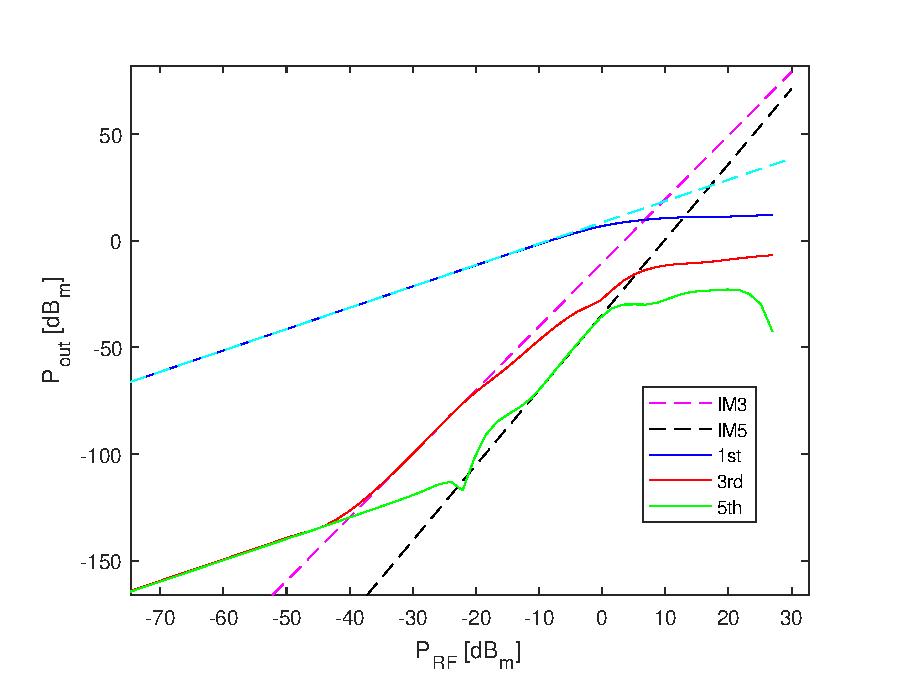
\includegraphics[scale=.75]{IIP3_schem_1tone}} \\
	\subfloat[][\emph{detail in IIP3 and IIP5}]{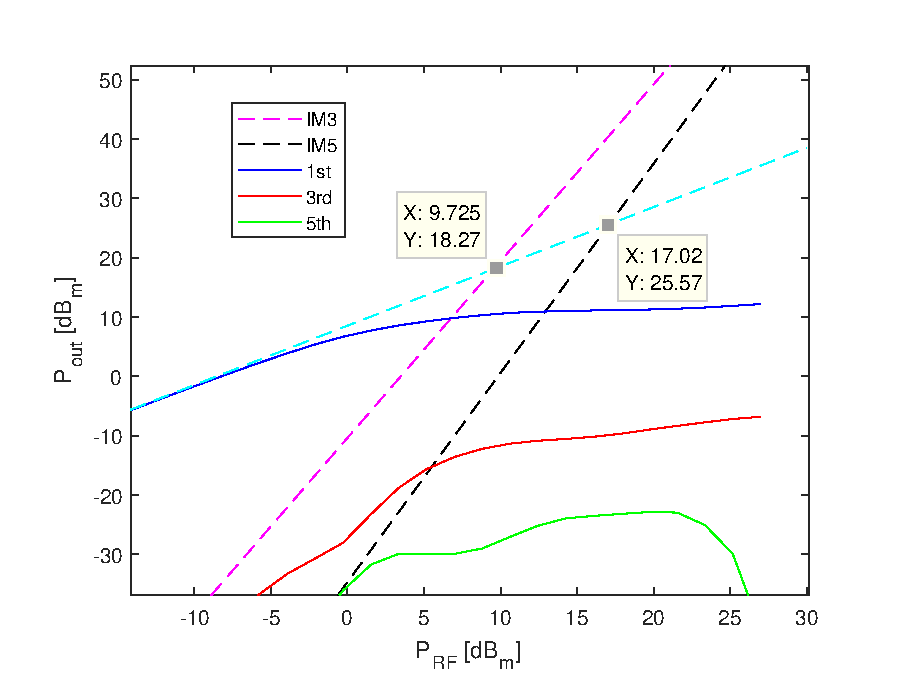
\includegraphics[scale=.75]{IIP3_schem_1tone_zoom}}
	\caption{Harmonics power, IIP\textsubscript{3} and IIP\textsubscript{5} in schematic, one tone analysis.}
	\label{fig:IIP3_1t_schem}
\end{figure}

\begin{figure}[H] 
	\centering
	\subfloat[][\emph{}]{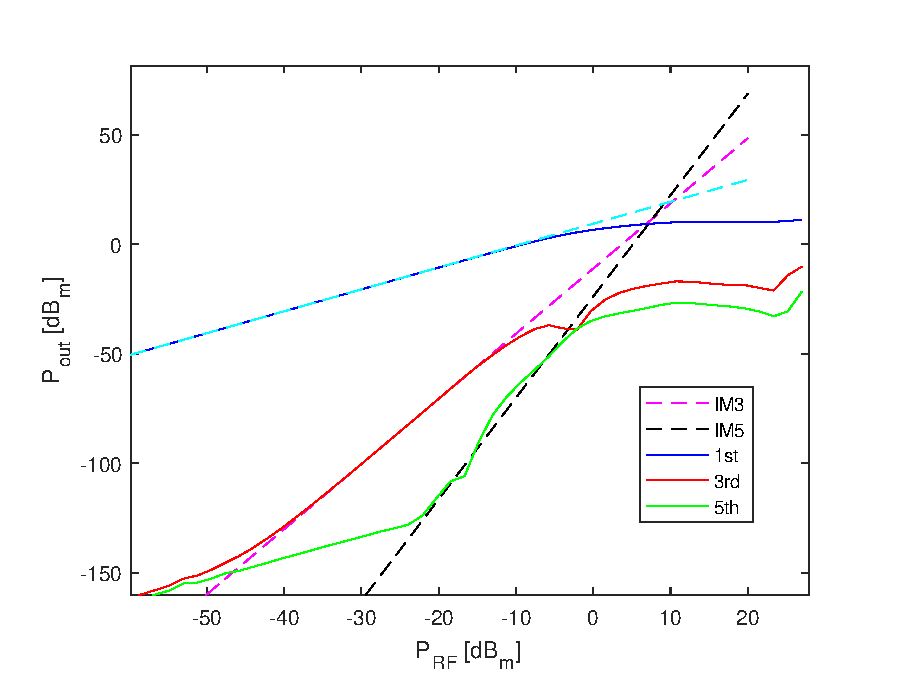
\includegraphics[scale=.75]{IIP3_layout_1tone}} \\
	\subfloat[][\emph{}]{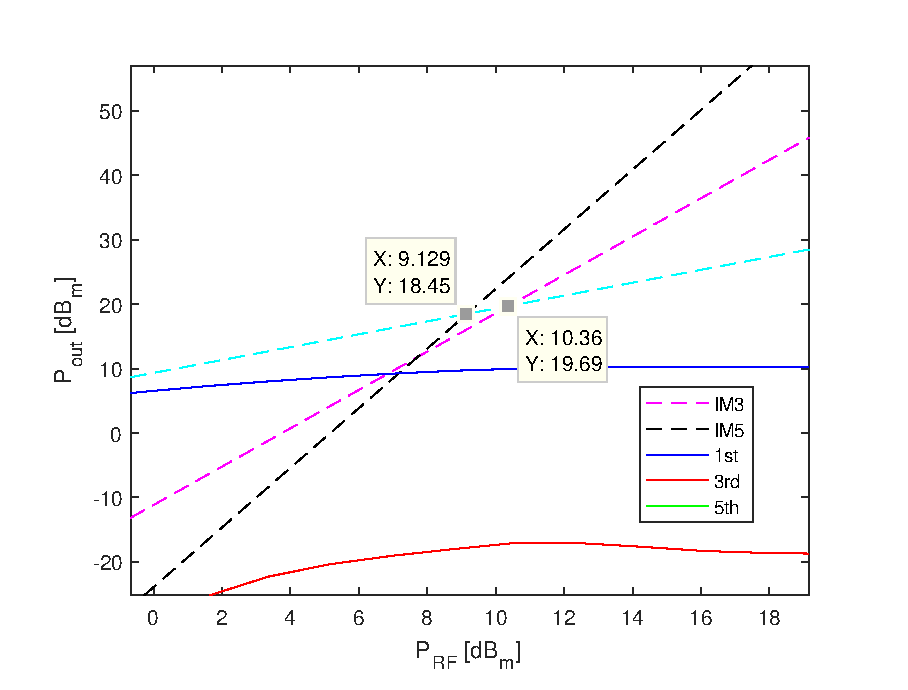
\includegraphics[scale=.75]{IIP3_layout_1tone_zoom}}
	\caption{IIP\textsubscript{3} and IIP\textsubscript{5} in layout, one tone analysis.}
	\label{fig:IIP3_1t_layout}
\end{figure}

\subsection{Two tone IM\textsubscript{3} and CIM\textsubscript{3} ratio}
In order to simulate the behaviour of a non-monochrome, fixed-bandwidth signal, the two tone analysis has been carried on. Two RF tones at f\textsubscript{RF}=110MHz and f\textsubscript{RF}\textsuperscript{'}=f\textsubscript{RF}+\(\delta\)f=111MHz have been adopted.
Figure \ref{fig:1dB_2tones} shows the 1dB compression point in this case.
Third order intermodulation frequency components result to be at \(9Mhz\) and \(12MHz\). Their behaviour along with increasing input power is shown in figure \ref{fig:IIP3_2t_schem}a and \ref{fig:IIP3_2t_schem}b. 
Graphs show that power related to fundamental is strongly reduced when two tones are injected, since power is spread among all intermodulation products. Being the power moved from the fundamental to IMPs, input and output intercepts point result lowered with respect the 1-tone case.

Frequency spectra at difference input power are shown in figure \ref{fig:DFT_2ton} and \ref{fig:DFT_2ton_zoom}. From the latter, informations about the carrier and third intermodulation data are selected. In particular, the 1dB compression point spectrum has been chosen (P\textsubscript{RF}=-9.68dB\textsubscript{m}), since this is set as the maximum input power accepted by the multiplier without heavy distortion. As it appears, power carried from fundamental tones (10MHz and 11MHz) barely increases after this point, whereas other tones keep increasing. Overall, the layout looks less performing as expected.

\begin{table} [H]
	\label{tab:IIP3_2tone}
	\caption{1dB compression point, IIP3 and CIM3 in two tones analysis.}
	\centering	
	\begin{tabular}{lccr} 
		\toprule 
		Parameter Name			& Schematic 	& Layout & unit \\ 
		\midrule
		\(P_{RF,1dB}\) & -8.01 & -9.68 & dB\(_{m}\)\\
		\(IIP_{3}\)  & 8.42 & 5.06 & dB\(_{m}\) \\
		\(OIP_{3}\)  & 16.9 &14.4 & dB\(_{m}\) \\
		\(CIM_{3,1dB}\) & 16.7 & 14.1 & dB \\
		\bottomrule 
	\end{tabular}	
\end{table}

\begin{figure}[H] 
	\centering
	\subfloat[][\emph{schematic}]{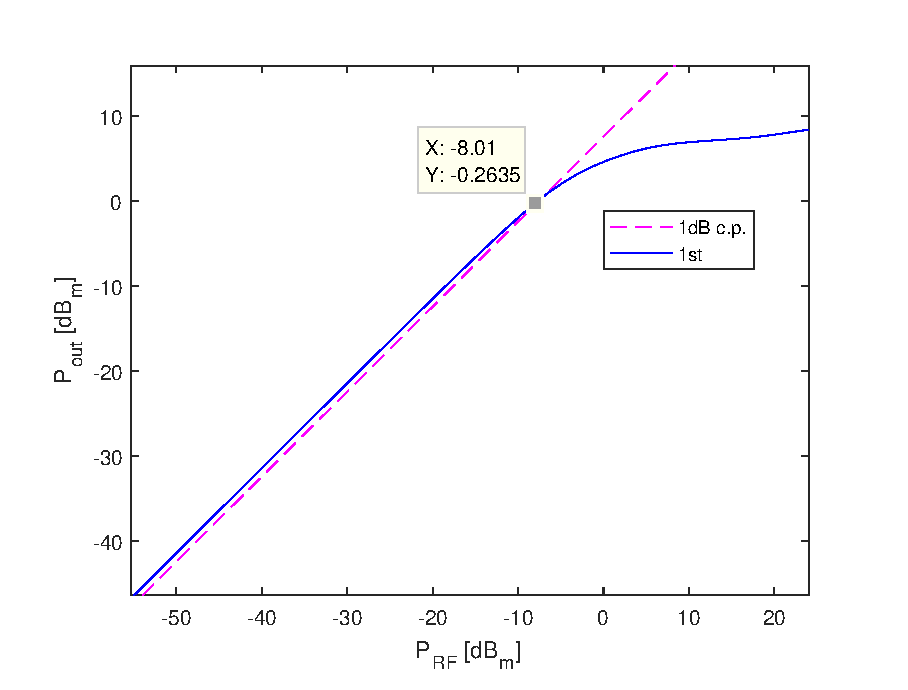
\includegraphics[scale=.7]{1dB_compression_2tone_schem}} \\
	\subfloat[][\emph{layout}]{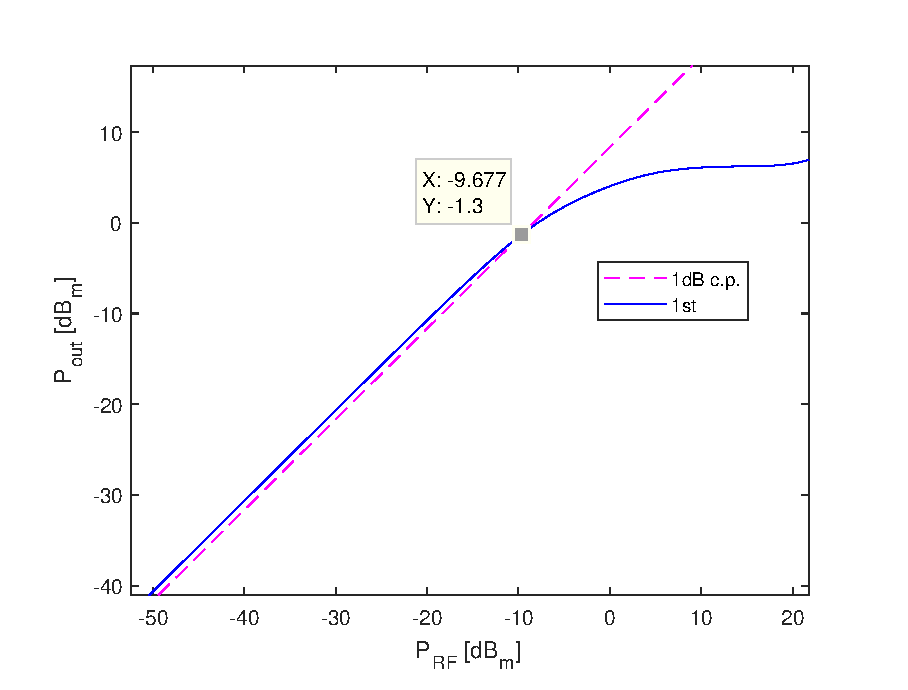
\includegraphics[scale=.7]{1dB_compression_2tone_layout}}
	\caption{1dB compression point, two tones.}
	\label{fig:1dB_2tones}
\end{figure}

\begin{figure}[H] 
	\centering
	\subfloat[][\emph{schematic}]{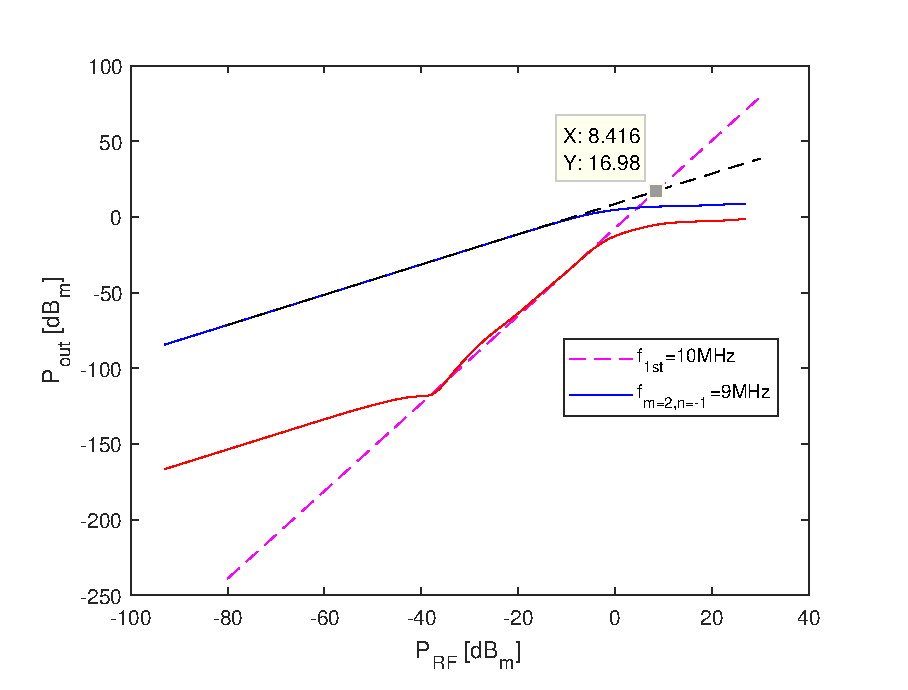
\includegraphics[scale=.7]{IIP3_schem_2tone}} \\
	\subfloat[][\emph{layout}]{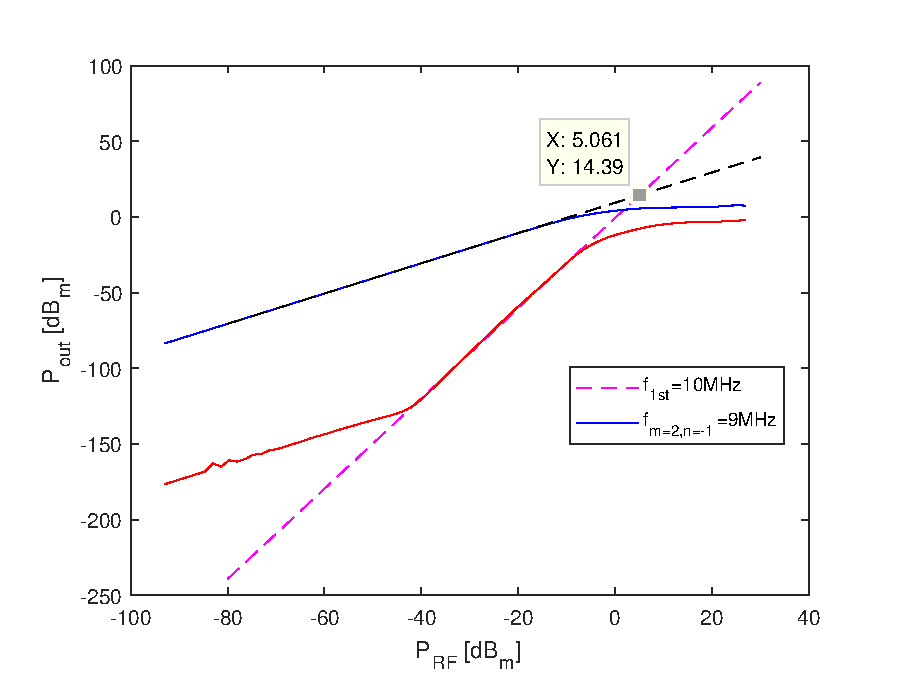
\includegraphics[scale=.7]{IIP3_layout_2tone}}
	\caption{Harmonics power, IIP\textsubscript{3} and IIP\textsubscript{5} in schematic, two tone analysis.}
	\label{fig:IIP3_2t_schem}
\end{figure}

\begin{figure}[H] 
	\centering
	\subfloat[][\emph{schematic}]{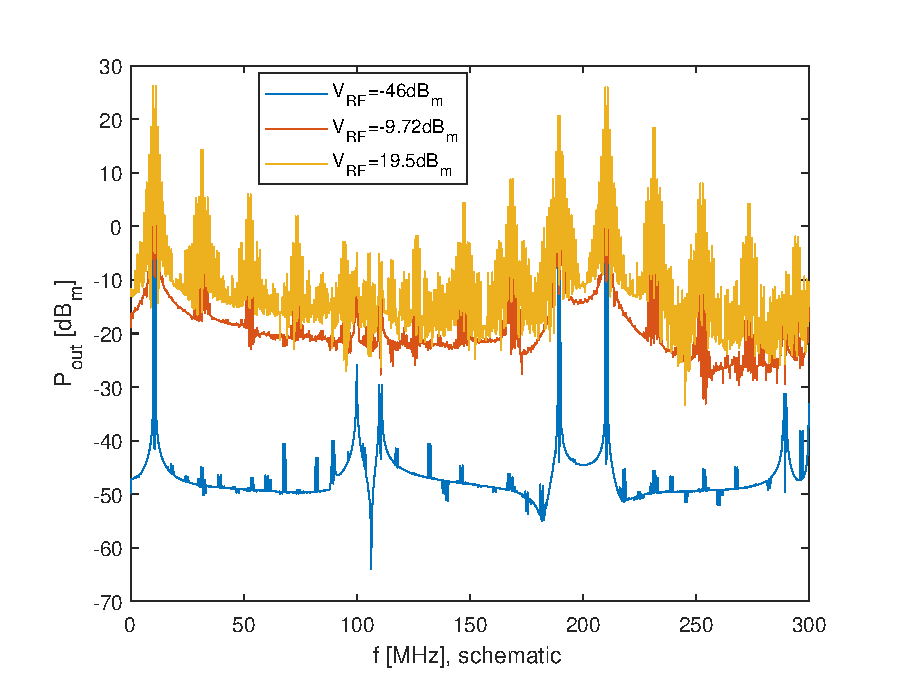
\includegraphics[scale=.7]{DFT_2tones_schem}} \\
	\subfloat[][\emph{layout}]{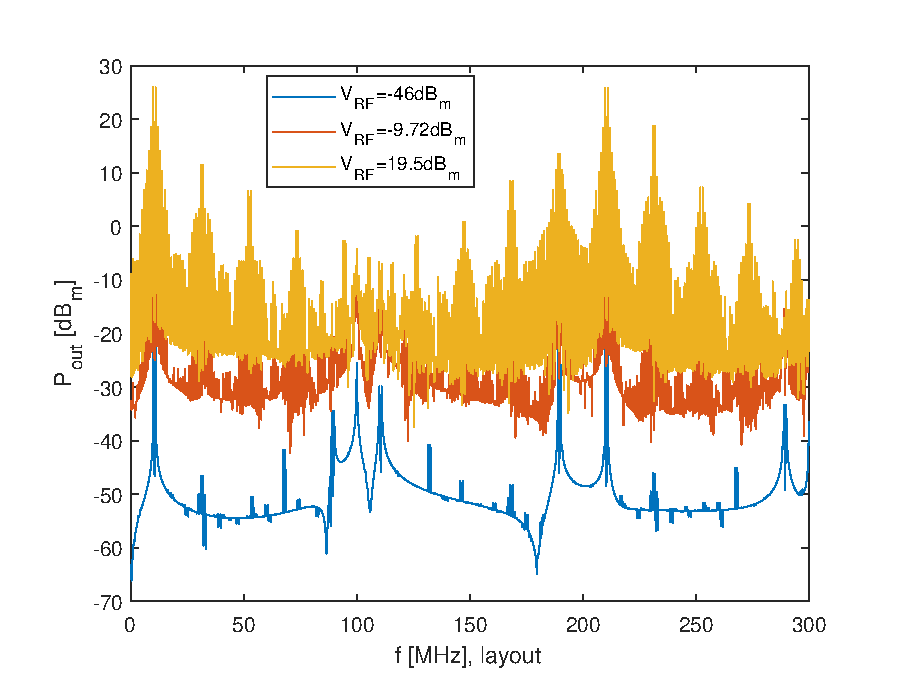
\includegraphics[scale=.7]{DFT_2tones_layout}}
	\caption{DFT, comparison between layout and schematic; cosine2 smoothing function.}
	\label{fig:DFT_2ton}
\end{figure}

\begin{figure}[H] 
	\centering
	\subfloat[][\emph{schematic}]{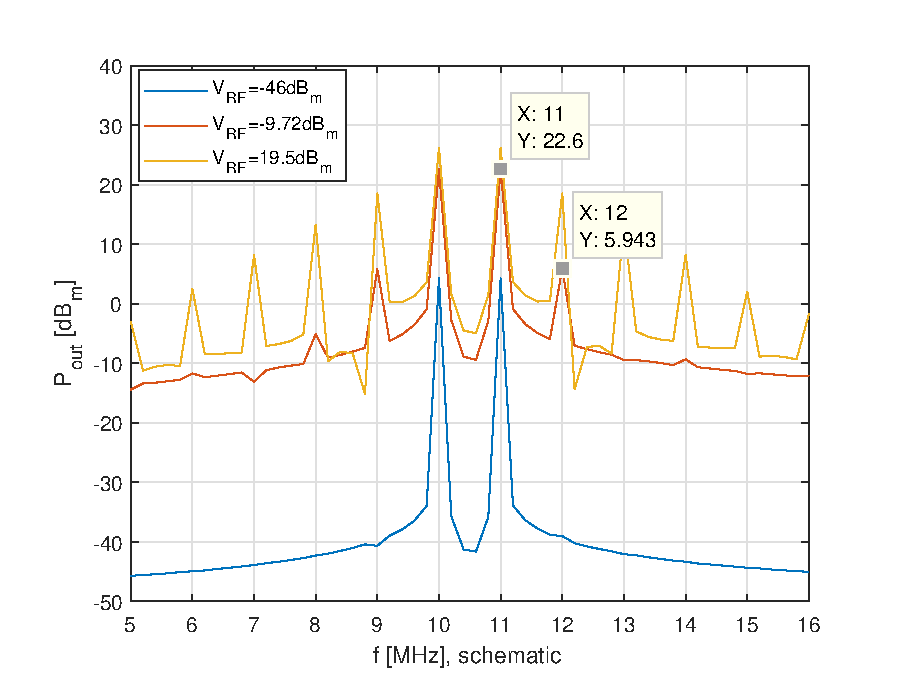
\includegraphics[scale=.7]{DFT_2tones_schem_zoom}} \\
	\subfloat[][\emph{layout}]{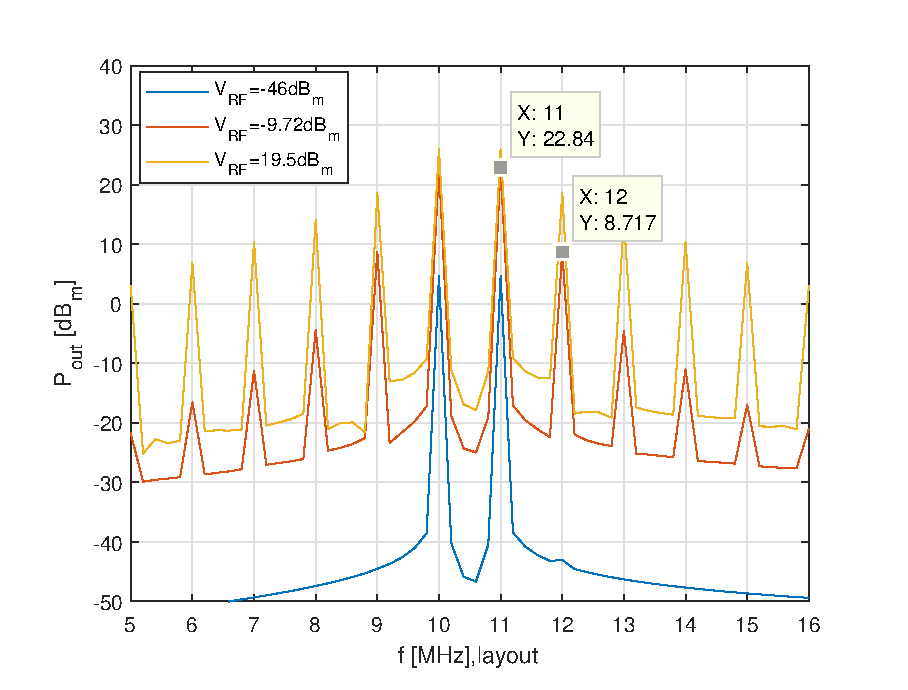
\includegraphics[scale=.7]{DFT_2tones_layout_zoom}}
	\caption{DFT, comparison between layout and schematic. CIM\textsubscript{3} measurement at 1dB compression point; cosine2 smoothing function. }
	\label{fig:DFT_2ton_zoom}
\end{figure}
